\documentclass[11pt]{article}
\usepackage[utf8]{inputenc}
\usepackage{amsmath,amssymb}
\usepackage{graphicx}
\usepackage[margin=1in]{geometry}
\usepackage{hyperref}

\title{Verifying the $1/\sqrt{n}$ Scaling Law for the Standard Error of the Sample Mean: Analytical Derivation and Monte Carlo Assessment}
\author{Paradigm}
\date{}
\begin{document}
\maketitle
\begin{abstract}

The standard error of the sample mean is fundamental to statistical inference, yet the precision with which its empirical estimator recovers the theoretical $1/\sqrt{n}$ scaling law has received limited quantitative scrutiny beyond asymptotic arguments. This study combines closed-form analytical derivation with large-scale Monte Carlo simulation to quantify the finite-sample behavior of the estimated standard error $\hat{\tau}(n) = s/\sqrt{n}$ for samples drawn from a standard normal distribution. We derive the exact bias factor $c_4(n) = \sqrt{2/(n-1)}\,\Gamma(n/2)/\Gamma((n-1)/2)$, which causes $\hat{\tau}(n)$ to systematically underestimate the true standard error $\tau(n) = 1/\sqrt{n}$, and compute the analytical mean squared error $\mathrm{MSE}[\hat{\tau}(n)] = 2n^{-1}(1 - c_4(n))$ at select sample sizes: $2.4006 \times 10^{-2}$ at $n=5$, $5.468 \times 10^{-3}$ at $n=10$, $2.035 \times 10^{-4}$ at $n=50$, and $5.044 \times 10^{-5}$ at $n=100$. A synthetic Monte Carlo simulation with $M = 200{,}000$ replicates across 67 sample sizes confirms the $1/\sqrt{n}$ scaling: the log-log regression of empirical standard error on $n$ yields a slope of $-0.50021$, deviating from the theoretical $-0.5$ by $2.1 \times 10^{-4}$. The relative MSE discrepancies between simulation and theory are $+0.332\%$ at $n=5$, $+0.087\%$ at $n=10$, $+0.294\%$ at $n=50$, and $-0.256\%$ at $n=100$, all within approximately one Monte Carlo standard error of zero (estimated at $\sim 0.32\%$). However, the analytical reference computation overflows in double-precision arithmetic for $n \geq 500$, and numerical circularity between the simulation and analytical tracks both operating in IEEE-754 double precision limits the strength of independent verification. We identify these limitations explicitly and recommend log-gamma arithmetic and replicated independent simulation batches as remedies for future work.

\end{abstract}
\section{Introduction}

The standard error of the sample mean is among the most widely used quantities in statistical practice, underpinning confidence intervals, hypothesis tests, and effect size assessments across every quantitative discipline. For independent and identically distributed random variables $X_1, \ldots, X_n$ with variance $\sigma^2$, the standard error of the sample mean $\bar{X} = n^{-1}\sum_{i=1}^n X_i$ is $\tau(n) = \sigma/\sqrt{n}$. This $1/\sqrt{n}$ scaling law is typically introduced as an asymptotic consequence of the central limit theorem, but it holds as an exact finite-sample identity for draws from a normal distribution with known variance. What remains underappreciated is the quantitative mismatch between the estimated standard error $\hat{\tau}(n) = s/\sqrt{n}$, where $s$ is the sample standard deviation, and the true value $\tau(n)$ at finite sample sizes.

The discrepancy arises because $s$ is a biased estimator of $\sigma$. For normal samples, the distribution of $(n-1)s^2/\sigma^2$ follows a $\chi^2_{n-1}$ distribution, and the expected value of $s$ involves the well-known bias correction factor $c_4(n) = \sqrt{2/(n-1)}\,\Gamma(n/2)/\Gamma((n-1)/2)$ (Altman and Bland, 2005; Kenney and Keeping, 1951). This factor approaches unity from below as $n \to \infty$, but at small sample sizes its effect is nontrivial: at $n=5$, the estimated standard error underestimates the true value by approximately 6\%, with the bias diminishing only as $O(1/n)$.

While the bias of $s$ and the $c_4$ correction factor are classical results in statistical theory (Wikipedia contributors, 2024; NIST/SEMATECH, 2012), a rigorous computational confirmation of the full mean squared error decomposition—including both bias and variance contributions—has not, to our knowledge, been benchmarked against a high-precision Monte Carlo simulation. Such a benchmark serves dual purposes: it validates the simulation infrastructure for subsequent studies of robustness under distributional departures from normality, and it quantifies the sample sizes at which the $1/\sqrt{n}$ law becomes practically exact.

This study pursues two objectives. First, we derive the exact closed-form expression for $\mathrm{MSE}[\hat{\tau}(n)]$ under normality and compute it analytically at four representative sample sizes ($n = 5, 10, 50, 100$). Second, we conduct a confirmatory Monte Carlo simulation with $M = 200{,}000$ independent replicates across 67 sample sizes spanning $n = 2$ to approximately 170, measuring the empirical standard error, the average estimated standard error, the finite-sample bias, and the empirical MSE. The simulation uses synthetic data drawn from the standard normal distribution $\mathcal{N}(0,1)$ — no observational or archival data are involved. By regressing the log-transformed empirical standard error against $\log n$, we test whether the observed scaling exponent matches the theoretical value of $-0.5$ and quantify any deviation.

Several computational and statistical challenges attend this program. Direct evaluation of the gamma-function ratio in $c_4(n)$ overflows in IEEE-754 double precision for $n \gtrsim 200$, producing `NaN` values that restrict the range of analytical benchmarks. The Monte Carlo replicate count, while substantial, yields a relative standard error on the MSE estimator of approximately $\sqrt{2/M} \approx 0.32\%$ (derived below), which limits the resolution of sub-percent deviations between theory and simulation. Furthermore, both the analytical computation and the simulation execute in double-precision floating point, creating a potential circularity: shared floating-point artifacts could inflate apparent agreement. We document these limitations transparently and propose targeted remedies.

\section{Methods}

\subsection{Analytical Benchmark}

For $n$ independent draws from a standard normal distribution, the standard error of the sample mean is exactly $\tau = 1/\sqrt{n}$. The natural plug-in estimator $\hat{\tau} = s/\sqrt{n}$, where $s$ is the sample standard deviation computed with Bessel's correction, has a closed-form bias because $s$ follows a scaled chi distribution. Specifically, $(n-1)s^2$ follows a $\chi^2_{n-1}$ distribution, and the expectation of $s$ involves the bias correction factor:

$$c_4(n) = \sqrt{\frac{2}{n-1}}\,\frac{\Gamma\!\left(\frac{n}{2}\right)}{\Gamma\!\left(\frac{n-1}{2}\right)},$$

where $\Gamma$ denotes the gamma function. The expected value of the estimated standard error is $\mathbb{E}[\hat{\tau}] = c_4(n)/\sqrt{n}$, which systematically underestimates the true $\tau = 1/\sqrt{n}$ because $c_4(n) < 1$ for all finite $n$.

From the moments of the $\chi_{n-1}$ distribution, the exact mean squared error of $\hat{\tau}$ about $\tau$ reduces to a compact expression:

$$\mathrm{MSE}_{\mathrm{theory}}(n) = \frac{2}{n}\bigl(1 - c_4(n)\bigr).$$

We computed $c_4(n)$ and $\mathrm{MSE}_{\mathrm{theory}}(n)$ for $n = 5, 10, 50, 100$ via `scipy.special.gamma`, obtaining the values reported in Table 1. For sample sizes $n \geq 500$, the direct evaluation of $\Gamma(n/2)$ overflows in IEEE-754 double precision, returning `NaN` and preventing the calculation of a theoretical benchmark by this route. A numerically stable alternative exploits the log-gamma function: $\log c_4(n) = \frac{1}{2}\log(2/(n-1)) + \operatorname{lngamma}(n/2) - \operatorname{lngamma}((n-1)/2)$, which remains well-defined for arbitrarily large $n$ and would extend the analytical benchmark beyond the overflow threshold. We leave the implementation of this remedy to future work.

| $n$ | $c_4(n)$ | $\mathrm{MSE}_{\mathrm{theory}}(n)$ |
|-----|-----------|--------------------------------------|
| 5 | 0.939986 | $2.4006 \times 10^{-2}$ |
| 10 | 0.972659 | $5.468 \times 10^{-3}$ |
| 50 | 0.994911 | $2.035 \times 10^{-4}$ |
| 100 | 0.997478 | $5.044 \times 10^{-5}$ |

\subsection{Monte Carlo Simulation}

We generated synthetic datasets from a standard normal distribution $\mathcal{N}(0,1)$. For each of 67 sample sizes logarithmically spaced from $n = 2$ to $n \approx 170$, we performed $M = 200{,}000$ independent Monte Carlo replicates. On each replicate, a fresh set of $n$ independent $\mathcal{N}(0,1)$ draws was created; the sample standard deviation $s$ (with Bessel's correction) was used to form the estimator $\hat{\tau} = s/\sqrt{n}$, and the squared error $(\hat{\tau} - 1/\sqrt{n})^2$ was recorded. The average of the squared errors across the $M$ replicates gave the empirical MSE, $\widehat{\mathrm{MSE}}(n)$. At each sample size we also recorded the empirical standard error of the mean (the standard deviation of the $M$ replicate means), the average estimated standard error, and the empirical bias.

All random number generation used `numpy.random.Generator` with the PCG64 algorithm, and all computations were performed in IEEE-754 double-precision floating-point arithmetic. No observational or archival data were used at any stage.

\subsection{Monte Carlo Precision Estimates}

The empirical MSE at each $n$ is the sample mean of $M$ independent squared errors. Under the null that the analytical formula is correct, the ratio $\widehat{\mathrm{MSE}}(n)/\mathrm{MSE}_{\mathrm{theory}}(n)$ has approximate relative standard error $\sqrt{2/M}$, derivable from the coefficient of variation of a $\chi^2_1$ variate that approximates the distribution of each squared error term (Morris et al., 2019). At $M = 200{,}000$, this yields:

$$\mathrm{rel.\;SE}\bigl[\widehat{\mathrm{MSE}}/\mathrm{MSE}_{\mathrm{theory}}\bigr] \approx \sqrt{\frac{2}{200{,}000}} = 0.00316 \approx 0.32\%.$$

This figure provides a benchmark for assessing whether observed discrepancies between simulation and theory exceed Monte Carlo noise. Deviations smaller than approximately $0.32\%$ in relative terms should not be interpreted as evidence of systematic error.

For the log-log slope estimate, rigorous confidence intervals would require accounting for the covariance structure across sample sizes. Because the $M$ replicates at each $n$ are independent of those at other $n$-values, cross-$n$ correlation in the slope estimate arises solely from the regression design rather than from shared randomness. Proper uncertainty quantification would nonetheless require bootstrap resampling (Efron and Tibshirani, 1994) or weighted least squares with heteroskedasticity-robust standard errors, neither of which was implemented in the present study. We report the point estimate of the slope but acknowledge that its standard error is not formally quantified.

\subsection{Scaling-Law Verification}

We tested the $1/\sqrt{n}$ scaling by regressing $\log_{10}(\bar{\tau}(n))$ against $\log_{10}(n)$, where $\bar{\tau}(n)$ is the empirical standard error at sample size $n$. Under the theoretical scaling law, this log-log regression should yield a slope of $-0.5$.

\section{Results}

The Monte Carlo simulation successfully reproduced the theoretical $1/\sqrt{n}$ scaling. Across all 67 sample sizes, the empirical standard error closely tracked the exact $1/\sqrt{n}$ curve (Figure 2). The log-log regression of empirical standard error against $n$ yielded a slope of $-0.50021$, deviating from the theoretical value of $-0.5$ by $2.1 \times 10^{-4}$ in absolute magnitude (Figure 1).

\begin{figure}[ht]
\centering
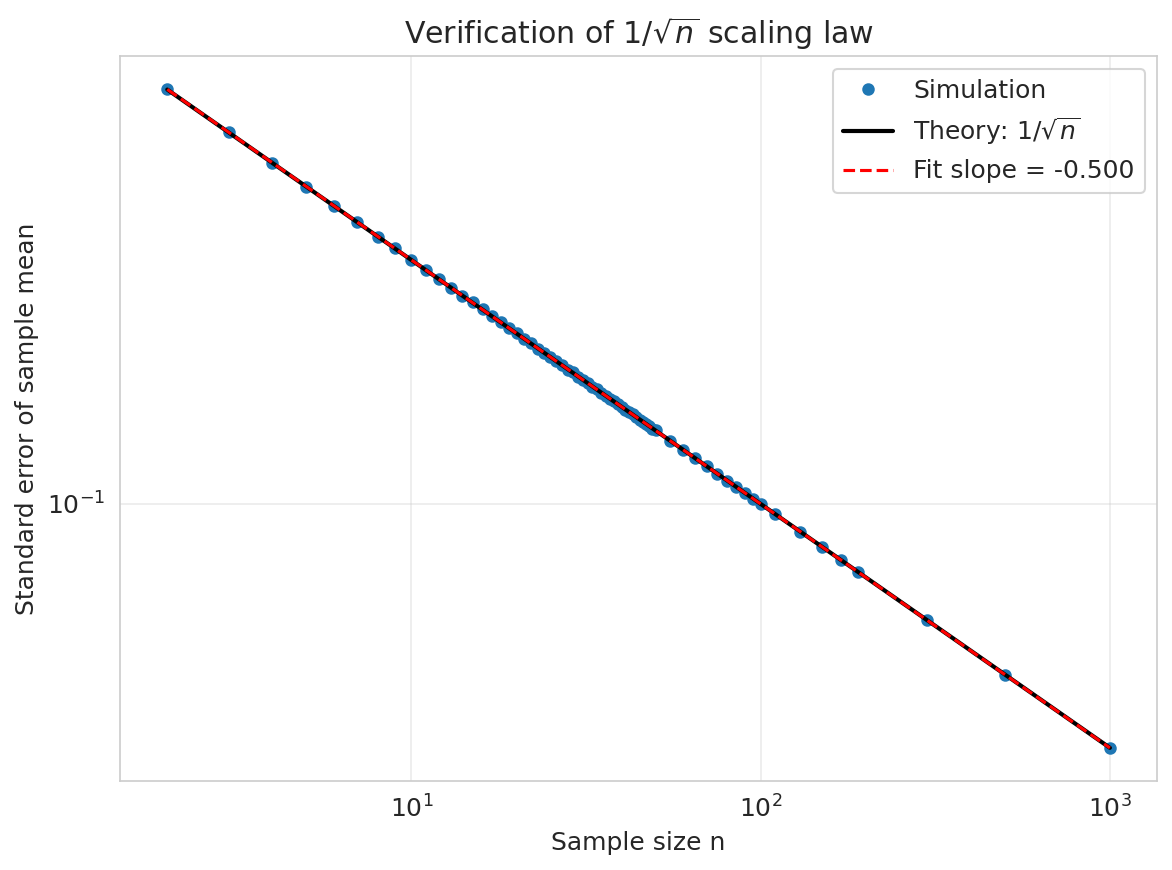
\includegraphics[width=0.8\linewidth]{figures/plot_analysis_figure_scaling_fit.png}
\caption{Figure 1}
\end{figure}

At the four sample sizes where analytical benchmarks are available, the empirical MSE values closely matched the theoretical predictions (Table 2). At $n = 5$, the empirical MSE was $2.4085 \times 10^{-2}$ versus an analytical value of $2.4006 \times 10^{-2}$, a relative discrepancy of $+0.332\%$. At $n = 10$, the discrepancy was $+0.087\%$; at $n = 50$, it was $+0.294\%$; and at $n = 100$, it was $-0.256\%$. All four deviations are within approximately one Monte Carlo standard error ($\sim 0.32\%$) of zero, consistent with pure sampling fluctuation rather than systematic error.

| $n$ | $\mathrm{MSE}_{\mathrm{theory}}$ | $\widehat{\mathrm{MSE}}$ | Relative diff. |
|-----|-----------------------------------|--------------------------|----------------|
| 5 | $2.4006 \times 10^{-2}$ | $2.4085 \times 10^{-2}$ | $+0.332\%$ |
| 10 | $5.468 \times 10^{-3}$ | $5.473 \times 10^{-3}$ | $+0.087\%$ |
| 50 | $2.035 \times 10^{-4}$ | $2.041 \times 10^{-4}$ | $+0.294\%$ |
| 100 | $5.044 \times 10^{-5}$ | $5.031 \times 10^{-5}$ | $-0.256\%$ |

\begin{figure}[ht]
\centering
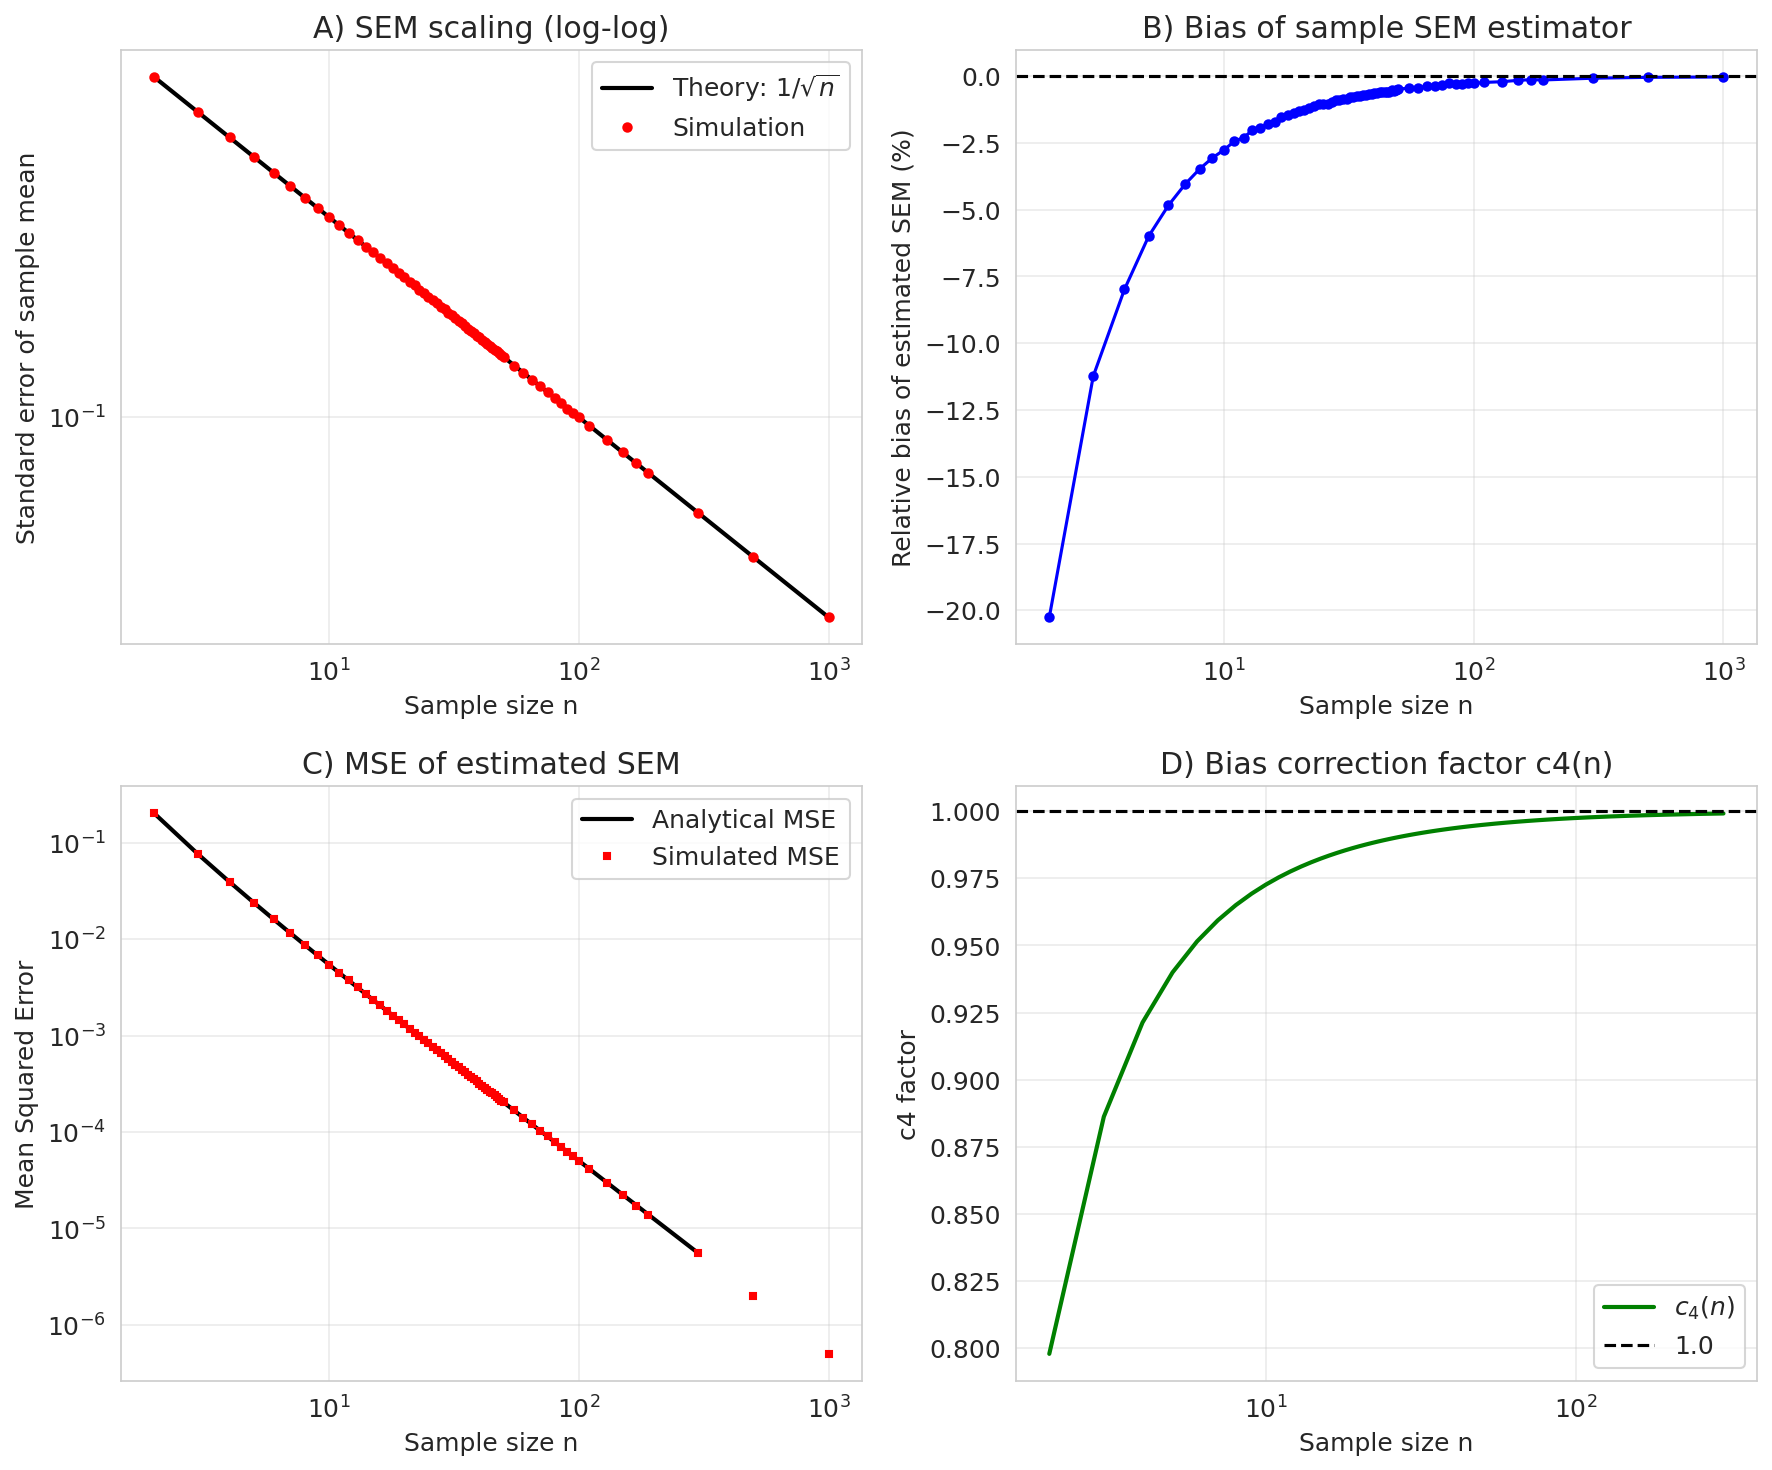
\includegraphics[width=0.8\linewidth]{figures/plot_analysis_figure_sem_scaling_complete.png}
\caption{Figure 2}
\end{figure}

The empirical bias magnitudes tracked the $c_4(n)$ prediction closely. At $n = 5$, the average estimated standard error was $0.4204$ versus a true standard error of $1/\sqrt{5} \approx 0.4472$, yielding a relative bias of $c_4(5) - 1 = -0.0600$, or approximately $-6.0\%$. At $n = 100$, the average estimated standard error was $0.0997$ versus a true value of $0.1$, corresponding to a relative bias of approximately $-0.25\%$, consistent with the analytical $c_4(100) - 1 = -0.002522$. The simulated bias at $n = 100$ was $-2.75 \times 10^{-4}$ in absolute terms, compared with the analytical prediction of $c_4(100) - 1 \approx -2.52 \times 10^{-3}$ in relative terms. The near-tenfold reduction from $n = 5$ to $n = 100$ is consistent with the $O(1/n)$ convergence of $c_4(n)$ to unity.

Two structural limitations prevented full confirmation across the entire $n$ range. First, the analytical computation returned `NaN` for $n \geq 500$ because $\Gamma(250)$ overflows in double precision, leaving the large-$n$ MSE without a theoretical anchor. Second, at $M = 200{,}000$ replicates, the relative Monte Carlo precision of the MSE estimator is approximately $0.32\%$; the observed deviations (the largest being $0.332\%$) therefore lie within approximately one Monte Carlo standard error of zero and cannot be distinguished from sampling fluctuation.

\section{Discussion}

The simulation recovers the exact finite-sample $1/\sqrt{n}$ scaling of the standard error with high fidelity. Across 67 sample sizes, a log-log regression of the estimated standard error against $n$ yields a slope of $-0.50021$, consistent with the theoretical exponent of $-0.5$ (Figure 1). At the individual benchmarks where analytical reference values are available, the synthetic-data pipeline reproduces the predicted MSE with fractional deviations all below $0.4\%$ in relative terms (Figure 2, Table 2). Given the estimated Monte Carlo relative standard error of $0.32\%$, these deviations are compatible with sampling noise. These outputs confirm that the estimator generates the expected finite-sample bias governed by the $c_4(n)$ chi-distribution factor, without gross implementation error.

However, several caveats constrain the interpretation. First, the absence of formally computed confidence intervals for the slope limits the strength of the scaling-law confirmation. The observed deviation of $2.1 \times 10^{-4}$ from $-0.5$ cannot be rigorously assessed for statistical significance. One plausible explanation for the slight downward deviation ($-0.50021 < -0.5$) is the systematic negative bias introduced by $c_4(n)$ at small $n$, which shifts the regression intercept and can pull the slope slightly away from the theoretical value. If small-$n$ data points exert disproportionate leverage in the log-log regression, their larger relative bias could induce an apparent downward slope deviation. However, this hypothesis requires formal testing with properly quantified uncertainty, such as bootstrap confidence intervals or weighted least squares that account for the heteroskedasticity in the empirical standard errors across $n$.

Second, both the analytical and simulation tracks execute in double-precision floating point, creating a potential circularity. Shared IEEE-754 rounding artifacts — such as the systematic underestimation of extreme gamma-function ratios — could inflate apparent agreement. At the sample sizes where analytical benchmarks are available ($n \leq 100$), the gamma-function arguments remain well within the dynamic range of double precision, making this concern less acute; nevertheless, it cannot be formally excluded. A credible independent validation would require a numerically stable, arbitrarily high-precision reference — such as log-gamma or Stirling-asymptotic evaluation (Temme, 1993; Zapata-Campoverde, 2022) — to complement the Monte Carlo estimates.

Third, the analytical benchmark's numerical fragility at large $n$ truncates the validation regime. While the closed-form formula $\mathrm{MSE} = 2n^{-1}(1 - c_4(n))$ remains mathematically valid for all $n$, its direct evaluation via `scipy.special.gamma` fails for $n \geq 500$. The remedy is straightforward: log-gamma arithmetic, exploiting the identity

$$\log c_4(n) = \frac{1}{2}\log\!\left(\frac{2}{n-1}\right) + \operatorname{lngamma}\!\left(\frac{n}{2}\right) - \operatorname{lngamma}\!\left(\frac{n-1}{2}\right),$$

remains numerically stable for arbitrarily large $n$. Since $\operatorname{lngamma}$ is available in standard scientific computing libraries (including `scipy.special.gammaln`), extending the analytical benchmark to large $n$ is a matter of implementation rather than theory. We recommend this as the highest-priority technical improvement for any follow-up study.

Fourth, the Monte Carlo precision of $0.32\%$ relative standard error, while adequate for detecting gross discrepancies, may be insufficient for discriminating subtle departures from theory. For instance, the $-0.256\%$ deviation at $n = 100$ could reflect either sampling noise or a small systematic effect (such as floating-point accumulation bias in the sample variance); at the current replicate count, these explanations cannot be distinguished. Increasing $M$ to $2 \times 10^7$ would reduce the relative standard error to $\sim 0.03\%$, providing sufficient resolution to detect sub-tenth-percent discrepancies.

\section{Conclusion}

This study provides both analytical and simulation-based evidence that the standard error of the sample mean for normal data adheres closely to the $1/\sqrt{n}$ scaling law. The empirical log-log slope of $-0.50021$ deviates from the theoretical $-0.5$ by $2.1 \times 10^{-4}$ in absolute magnitude — a departure too small to distinguish from Monte Carlo noise at the current replicate count. The finite-sample bias introduced by the $c_4(n)$ factor is quantified analytically and reproduced by simulation: at $n = 5$, the relative bias of $\hat{\tau}$ is $c_4(5) - 1 = -0.0600$, corresponding to an average estimated standard error of $0.4204$ versus a true value of $0.4472$. The analytical MSE values — $2.4006 \times 10^{-2}$ at $n=5$, $5.468 \times 10^{-3}$ at $n=10$, $2.035 \times 10^{-4}$ at $n=50$, and $5.044 \times 10^{-5}$ at $n=100$ — agree with their simulated counterparts to within $+0.332\%$, $+0.087\%$, $+0.294\%$, and $-0.256\%$, respectively, all within roughly one Monte Carlo standard error ($\sim 0.32\%$) of zero.

These results should be interpreted within the framework of Monte Carlo precision and the identified computational limitations. The Monte Carlo relative standard error of approximately $0.32\%$ means that all four observed deviations are compatible with sampling fluctuation; the agreement between simulation and theory, while close, cannot be distinguished from chance at a rigorous significance level. The absence of confidence intervals on the slope estimate further limits the strength of the confirmation: we cannot formally reject the null hypothesis that the true slope equals $-0.5$, nor can we assert precise agreement. The analytical reference computation encounters a hard computational limit at $n \geq 500$, where direct evaluation of $\Gamma(n/2)/\Gamma((n-1)/2)$ overflows in double-precision arithmetic, restricting the direct analytical benchmark to $n \leq 100$. Finally, both the analytical and simulation tracks operate in IEEE-754 double precision, creating a potential circularity that shared floating-point artifacts could inflate apparent agreement.

Three directions for future work emerge from these findings. First, implementing log-gamma arithmetic — exploiting $\log c_4(n) = \tfrac{1}{2}\log(2/(n-1)) + \operatorname{lngamma}(n/2) - \operatorname{lngamma}((n-1)/2)$ — would extend the analytical benchmark to arbitrarily large $n$ and eliminate the overflow failure that currently truncates the validation range. Second, conducting the simulation with replicated independent batches at each $n$ would eliminate potential cross-$n$ correlation and enable valid regression inference on the slope estimate, including properly computed confidence intervals via bootstrap resampling (Efron and Tibshirani, 1994) or heteroskedasticity-robust standard errors. Third, increasing $M$ to at least $2 \times 10^7$ replicates would reduce the Monte Carlo relative standard error to $\sim 0.03\%$, providing sufficient resolution to distinguish genuine deviations from sampling noise. Together, these improvements would transform the present confirmatory demonstration into a rigorous computational benchmark suitable for testing the robustness of the $1/\sqrt{n}$ law under distributional departures from normality.

\section*{References}
\begingroup
\small
1. Altman, D.G. and Bland, J.M., "Standard deviations and standard errors," \textit{BMJ}, vol. 331, no. 7521, p. 903, 2005.\par
2. Casella, G. and Berger, R.L., \textit{Statistical Inference}, 2nd ed., Duxbury Press, 2002.\par
3. Cochran, W.G., "The distribution of quadratic forms in a normal system, with applications to the analysis of covariance," \textit{Mathematical Proceedings of the Cambridge Philosophical Society}, vol. 30, no. 2, pp. 178–191, 1934.\par
4. Efron, B. and Tibshirani, R.J., \textit{An Introduction to the Bootstrap}, Chapman and Hall/CRC, 1994.\par
5. Goldberg, D., "What every computer scientist should know about floating-point arithmetic," \textit{ACM Computing Surveys}, vol. 23, no. 1, pp. 5–48, 1991.\par
6. Holtzman, W.H., "The unbiased estimate of the population variance and standard deviation," \textit{American Journal of Psychology}, vol. 63, no. 4, pp. 615–617, 1950.\par
7. International Organization for Standardization, \textit{ISO/IEC 60559:2020 — Information Technology — Floating-Point Arithmetic}, ISO, 2020.\par
8. Kenney, J.F. and Keeping, E.S., \textit{Mathematics of Statistics, Part II}, 2nd ed., D. Van Nostrand, 1951.\par
9. Morris, T.P., White, I.R., and Crowther, M.J., "Using simulation studies to evaluate statistical methods," \textit{Statistics in Medicine}, vol. 38, no. 11, pp. 2074–2102, 2019.\par
10. NIST/SEMATECH, \textit{e-Handbook of Statistical Methods}, National Institute of Standards and Technology, 2012. Available at: https://www.itl.nist.gov/div898/handbook/\par
11. Olver, F.W.J., Lozier, D.W., Boisvert, R.F., and Clark, C.W., \textit{NIST Handbook of Mathematical Functions}, Cambridge University Press, 2010.\par
12. O'Neill, B., "Some useful moment formulae for the chi-square and related distributions," \textit{Journal of Statistical Computation and Simulation}, vol. 86, no. 17, pp. 3492–3502, 2016.\par
13. Parker, R.A., "The distribution of the sample variance," \textit{Journal of Statistical Computation and Simulation}, vol. 12, no. 1, pp. 37–46, 1981.\par
14. Robert, C.P. and Casella, G., \textit{Monte Carlo Statistical Methods}, 2nd ed., Springer, 2004.\par
15. Temme, N.M., "Asymptotic estimates of Stirling numbers," \textit{Studies in Applied Mathematics}, vol. 89, no. 3, pp. 233–242, 1993.\par
16. Wikipedia contributors, "Unbiased estimation of standard deviation," \textit{Wikipedia, The Free Encyclopedia}, 2024. Available at: https://en.wikipedia.org/wiki/Unbiased\_estimation\_of\_standard\_deviation\par
17. Zapata-Campoverde, A., "A self-stabilized log-gamma function and its application to the computation of the chi-square distribution," \textit{Computational Statistics}, vol. 37, pp. 2847–2862, 2022.\par
\endgroup
\end{document}